\documentclass[final]{beamer}
\mode<presentation>{\usetheme{I6pd}}

\usepackage[english]{babel}
\usepackage[orientation=landscape,size=a0]{beamerposter}

\usepackage{color}
\usepackage{complexity}

\newcommand{\emphblue}[1]{\emph{\textcolor{blue}{#1}}}
\newcommand{\sigmastar}{\Sigma^*}
\newcommand{\kr}{\leq_{ker}^p}
\newcommand{\mor}{\leq_{m}^p}

\title{On the computational complexity of equivalence relations}
\author{Jeffrey Finkelstein}
\institute{Tufts University}
\date{\today}

\begin{document}
\begin{frame}{}
  \begin{columns}[t]

    %% left column
    \begin{column}{.3\linewidth}

      \begin{block}{\LARGE What is an equivalence relation?}
        \Large
        \begin{itemize}
        \item Let $\sigmastar=\{0,1\}^*$. Then
          $R\subseteq\sigmastar\times\sigmastar$ is an \emphblue{equivalence
          relation} if the following properties hold for all
          $x,y,z\in\sigmastar$:
          \begin{list}
            \Large
          \item i. (\emphblue{reflexivity}) $(x,x)\in R$
          \item ii. (\emphblue{symmetry}) $(x,y)\in R\implies (y,x)\in R$
          \item iii. (\emphblue{transitivity}) if $(x,y)\in R$ and $(y,z)\in
            R$, then $(x,z)\in R$
          \end{list}
          If $(x,y)\in R$, we use the notation $x\sim y$ and say \emph{$x$
            relates to $y$}.
        \item $\PEq=\{R\subseteq\sigmastar\times\sigmastar|R$ is an equivalence
          relation for which membership can be \emphblue{decided} by a
          deterministic Turing machine in polynomial time$\}$
        \item $\NPEq=\{R\subseteq\sigmastar\times\sigmastar|R$ is an
          equivalence relation for which membership can be \emphblue{verified}
          by a deterministic Turing machine in polynomial time$\}$
        \end{itemize}
      \end{block}

      \begin{block}{\LARGE How hard are equivalence relations?}
        \Large
        \begin{itemize}
          \setlength{\itemsep}{20pt}
        \item in \PEq:
          \begin{itemize}\Large
          \item \emphblue{the equality relation}: are two strings equal?
          \item \emphblue{same parity}: do two strings have the same parity
            (even or odd number of ones)?
          \item \emphblue{same bitcount}: do two strings have the same number
            of ones?
          \item \emphblue{equal or complement}: are two strings either equal or
            bitwise complements?
          \item \emphblue{tree isomorphism}: are two trees the same up to a
            relabeling of vertices?
          \end{itemize}
        \item in $\NPEq$ (not known to be in \PEq):
          \begin{itemize}\Large
          \item \emphblue{graph isomorphism}: are two graphs the same up to a
            relabeling of vertices?
          \item \emphblue{context-free grammar isomorphism}: do two context
            free grammars produce the same language?
          \item \emphblue{algebraic structure isomorphism}: given two algebraic
            structures, are they the same up to relabeling of elements?
            %\item these problems are actually all of equivalent complexity!
          \end{itemize}
        \item really hard (not known to be in \NPEq):
          \begin{itemize}\Large
          \item \emphblue{boolean formula isomorphism}: are two boolean
            formulas the same up to a permutation of input variables?
          \end{itemize}
        \end{itemize}
      \end{block}

      \begin{block}{\LARGE Why are equivalence relations important?}
        \begin{itemize}
          \Large
        \item graph isomorphism is a candidate for $\NP\backslash\P$ (worth
          \$1,000,000!)
        \item as a tool for studying other complexity classes
        \item applications in determining equivalence of structures in
          practical computer science and engineering
        \end{itemize}
      \end{block}
    \end{column}

    %% middle column
    \begin{column}{.3\linewidth}
      \begin{block}{\LARGE Kernel reduction between equivalence relation}
        \Large In this figure the polynomial time computable function $f$ maps
        binary strings to graphs such that if $a$ and $b$ are binary strings
        with the same number of ones, then $f(a)$ is isomorphic to $f(b)$. In
        this specific example, $x$ and $y$ both have three ones and 
        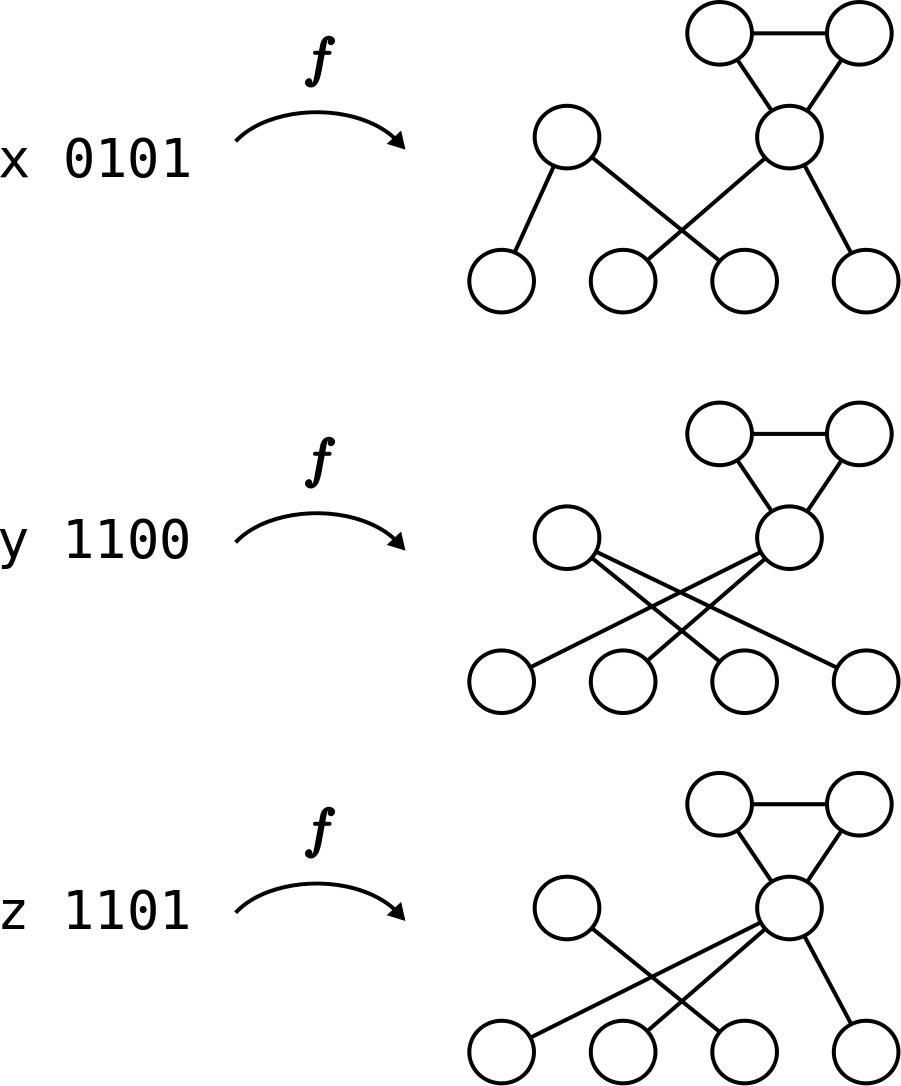
\includegraphics{images/rbc_gi}
      \end{block}
    \end{column}

    %% right column
    \begin{column}{.3\linewidth}
      \begin{block}{\LARGE What is a kernel reduction?}
        \begin{itemize}\Large
        \item if $R,S$ are equivalence relations and $\exists f\in\FP: (x,y)\in
          R\iff(f(x),f(y))\in S$, then we say $R$ \emphblue{kernel reduces} to
          $S$, and we write $R\kr S$
        \item if $\exists f\in\FP: (x,y)\in R\iff f(x,y)\in S$, then we say $R$
          \emphblue{many-one reduces} to $S$, and we write $R\mor S$
        \item kernel reduction is \emphblue{less powerful} than many-one
          reduction, but \emphblue{more natural} for equivalence relations
        \item \textbf{Lemma:} $R\kr S\implies R\mor S$
        \item if $R\in\PEq$ and $\forall S\in\PEq$, $S\kr R$, then we say $R$
          is \emphblue{\PEq-complete}
        \item \textbf{Theorem:} if $R$ is \NPEq-complete then $R$ is
          \NP-complete
        \end{itemize}
      \end{block}

      \begin{block}{\LARGE What do kernel reductions look like?}
        \begin{itemize}\Large
        \item most known reductions between \emphblue{equivalence problems in
          $\NPEq$} and \emphblue{graph isomorphism} are kernel reductions
        \item many equivalence problems in $\PEq$ reduce to equality
        \item maps a \emphblue{single object} in one category to a
          \emphblue{single object} in another category (does not map pairs)
        \end{itemize}
      \end{block}

      \begin{block}{\LARGE What do we want to study about kernel reductions?}
        \begin{itemize}\Large
        \item questions to address:
          \begin{itemize}\Large
          \item are kernel reductions \emphblue{different} from many-one
            reductions?
          \item are there \PEq-complete problems? are there \NPEq-complete
            problems?
          \item is the \emphblue{equality relation} \PEq-complete?
          \item what is the relationship between \NP-complete problems and
            \NPEq-complete problems?
          \end{itemize}
        \end{itemize}
      \end{block}

    \end{column}

  \end{columns}
\end{frame}

\end{document}
